% allgem. Dokumentenformat
\documentclass[a4paper,12pt,headsepline]{scrartcl}
%Variablen welche innerhalb der gesamten Arbeit zur Verfügung stehen sollen
\newcommand{\titleDocument}{Bachelor Thesis}
\newcommand{\subjectDocument}{in Computer Science}


\newcommand{\specialcell}[2][c]{%
	\begin{tabular}[#1]{c}
		#2
	\end{tabular}
}

\newcommand{\specialcellleft}[2][@{}l]{%
	\begin{tabular}[#1]{@{}l}
		#2
	\end{tabular}
}

\newcommand{\fixme}[1]{
	~\\
	\noindent
	\textbf{\textcolor{red}{FIXME: #1}}
	\\
}




% weitere Pakete
% Grafiken aus PNG Dateien einbinden
\usepackage{graphicx}

% Eurozeichen einbinden
\usepackage[right]{eurosym}

% Umlaute unter UTF8 nutzen
\usepackage[utf8]{inputenc}

% Zeichenencoding
\usepackage[T1]{fontenc}

\usepackage{lmodern}
\usepackage{fix-cm}

% floatende Bilder ermöglichen
%\usepackage{floatflt}

% mehrseitige Tabellen ermöglichen
\usepackage{longtable}

% Unterstützung für Schriftarten
%\newcommand{\changefont}[3]{ 
%\fontfamily{#1} \fontseries{#2} \fontshape{#3} \selectfont}

% Packet für Seitenrandabständex und Einstellung für Seitenränder
\usepackage{geometry}
\geometry{left=3.5cm, right=2cm, top=2.5cm, bottom=2cm}

% Paket für Boxen im Text
\usepackage{fancybox}

% bricht lange URLs "schoen" um
\usepackage[hyphens,obeyspaces,spaces]{url}

% Paket für Textfarben
\usepackage{color}

% Mathematische Symbole importieren
\usepackage{amssymb}

% auf jeder Seite eine Überschrift (alt, zentriert)
%\pagestyle{headings}

% erzeugt Inhaltsverzeichnis mit Querverweisen zu den Kapiteln (PDF Version)
\usepackage[bookmarksnumbered,pdftitle={\titleDocument},hyperfootnotes=false]{hyperref} 
%\hypersetup{colorlinks, citecolor=red, linkcolor=blue, urlcolor=black}
%\hypersetup{colorlinks, citecolor=black, linkcolor= black, urlcolor=black}

% neue Kopfzeilen mit fancypaket
\usepackage{fancyhdr} %Paket laden
\pagestyle{fancy} %eigener Seitenstil
\fancyhf{} %alle Kopf- und Fußzeilenfelder bereinigen
\fancyhead[L]{\nouppercase{\leftmark}} %Kopfzeile links
\fancyhead[C]{} %zentrierte Kopfzeile
\fancyhead[R]{\thepage} %Kopfzeile rechts
\renewcommand{\headrulewidth}{0.4pt} %obere Trennlinie
%\fancyfoot[C]{\thepage} %Seitennummer
%\renewcommand{\footrulewidth}{0.4pt} %untere Trennlinie

% für Tabellen
\usepackage{array}

% Runde Klammern für Zitate
%\usepackage[numbers,round]{natbib}

% Festlegung Art der Zitierung - Havardmethode: Abkuerzung Autor + Jahr
\bibliographystyle{alphadin}

% Schaltet den zusätzlichen Zwischenraum ab, den LaTeX normalerweise nach einem Satzzeichen einfügt.
\frenchspacing

% Paket für Zeilenabstand
\usepackage{setspace}

% für Bildbezeichner
\usepackage{capt-of}

% für Stichwortverzeichnis
\usepackage{makeidx}

% für Listings
\usepackage{listings}
\lstset{numbers=left, numberstyle=\tiny, numbersep=5pt, keywordstyle=\color{black}\bfseries, stringstyle=\ttfamily,showstringspaces=false,basicstyle=\footnotesize,captionpos=b}
\lstset{language=java}

% Indexerstellung
\makeindex

% Abkürzungsverzeichnis
\usepackage[german]{nomencl}
\let\abbrev\nomenclature

% Abkürzungsverzeichnis LiveTex Version
\renewcommand{\nomname}{Abkürzungsverzeichnis}
\setlength{\nomlabelwidth}{.25\hsize}
\renewcommand{\nomlabel}[1]{#1 \dotfill}
\setlength{\nomitemsep}{-\parsep}
\makenomenclature
%\makeglossary

% Abkürzungsverzeichnis TeTEX Version
% \usepackage[german]{nomencl}
% \makenomenclature
% %\makeglossary
% \renewcommand{\nomname}{Abkürzungsverzeichnis}
% \setlength{\nomlabelwidth}{.25\hsize}
% \renewcommand{\nomlabel}[1]{#1 \dotfill}
% \setlength{\nomitemsep}{-\parsep}

% Disable single lines at the start of a paragraph (Schusterjungen)
\clubpenalty = 10000
% Disable single lines at the end of a paragraph (Hurenkinder)
\widowpenalty = 10000
\displaywidowpenalty = 10000

\begin{document}
% hier werden die Trennvorschläge inkludiert
%hier müssen alle Wörter rein, welche Latex von sich auch nicht korrekt trennt bzw. bei denen man die genaue Trennung vorgeben möchte
\hyphenation{
Film-pro-du-zen-ten
Lux-em-burg
Soft-ware-bau-steins
zeit-in-ten-siv
}

%Schriftart Helvetica
%\changefont{phv}{m}{n}

% Leere Seite am Anfang
\newpage
\thispagestyle{empty} % erzeugt Seite ohne Kopf- / Fusszeile
\section*{ }

% Titelseite %
% das Papierformat zuerst
%\documentclass[a4paper, 11pt]{article}

% deutsche Silbentrennung
%\usepackage[ngerman]{babel}

% wegen deutschen Umlauten
%\usepackage[ansinew]{inputenc}

% hier beginnt das Dokument
%\begin{document}


\thispagestyle{empty}

%\begin{figure}[t]
% \includegraphics[width=0.6\textwidth]{abb/fh_koeln_logo}
%\end{figure}

\begin{figure}[t]
 \centering
 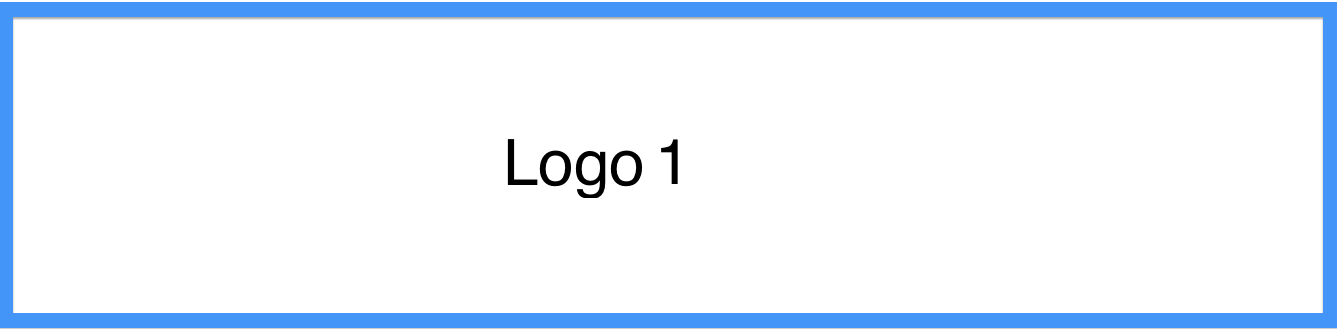
\includegraphics[width=0.6\textwidth]{abb/logo1}
~~~~~~~~~~
 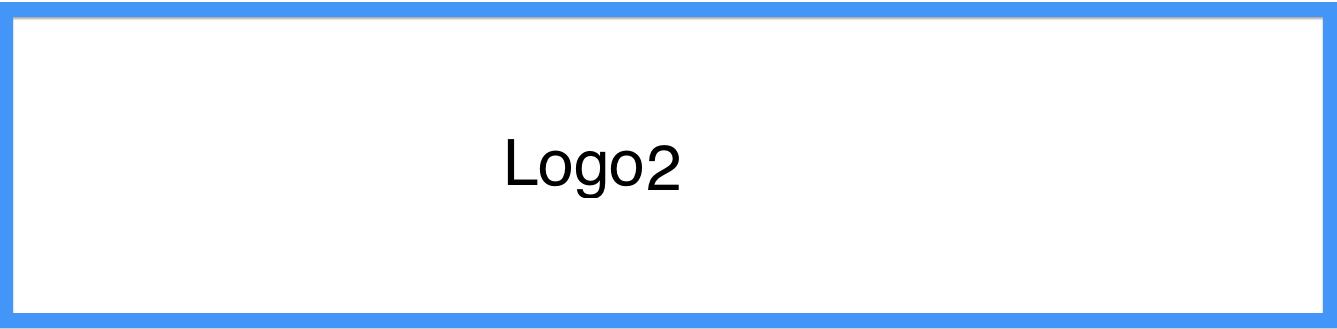
\includegraphics[width=0.20\textwidth]{abb/logo2}
\end{figure}


\begin{verbatim}


\end{verbatim}

\begin{center}
\Large{University of Bayreuth}\\
\end{center}


\begin{center}
\Large{Institute for Computer Science}
\end{center}
\begin{verbatim}








\end{verbatim}
\begin{center}
\doublespacing
\textbf{\LARGE{\titleDocument}}\\
\singlespacing
\begin{verbatim}

\end{verbatim}
\textbf{{~\subjectDocument}}
\end{center}
\begin{verbatim}

\end{verbatim}
\begin{center}

\end{center}
\begin{verbatim}






\end{verbatim}
\begin{flushleft}
\begin{tabular}{llll}
\textbf{Topic:} & & Integration of JPA-conform ORM-Implementations & \\
	& & in Hibernate Search & \\
& & \\
\textbf{Author:} & & Martin Braun <martinbraun123@aol.com>& \\
& & Matrikel-Nr. 1249080 & \\
& & \\
\textbf{Version date:} & & \today &\\
& & \\
\textbf{1. Supervisor:} & & Prof. Dr. Stefan Jablonski &\\
\textbf{2. Supervisor:} & & Prof. Dr. Bernhard Westfechtel &\\
\end{tabular}
\end{flushleft}
%
%\pagebreak
%~
%\pagebreak

%\begin{verbatim}






















%\end{verbatim}

%\begin{center}
%	To my parents.
%\end{center}

%\afterpage{\null\newpage}
%\pagebreak
%~\\\\
%\pagebreak
%~

% römische Numerierung
%\pagenumbering{arabic}

% 1.5 facher Zeilenabstand
\onehalfspacing

% Einleitung / Abstract
% !TeX spellcheck = en_GB
\section*{Abstract}

Fulltext search engines are a powerful tool to improve query results in applications where relational databases don't suffice. However, they don't integrate well with the widely spread concept of object relationship mappers (ORM, in Java predominantly represented by the standard JPA) in the object oriented programming world.
\\\\
This is where Hibernate Search comes into use for Java developers: It combines JPA and fulltext search by being the intermediary between Hibernate ORM and a Lucene based fulltext index. It has one problem though: Hibernate Search only works with Hibernate ORM but not with other JPA-conform providers even though it is possible to support these. In this thesis we will show how such a generic version can be accomplished.
\\\\
After discussing the methods we use, we give an explanation why a generic Hibernate Search is a desirable solution for JPA developers. Creating it is challenging as we have to build a standalone version of Hibernate Search's internal engine first and then integrate it with JPA together with an automatic index updating mechanism. We solve these challenges and give a usage example of the completed generic version. Finally, we discuss the current development state of the generic version and give an outlook on the planned merging process with the original Hibernate Search.

\pagebreak

\section*{Zusammenfassung}
Volltextsuchengines sind ein wertvolles Werkzeug um Suchergebnisse in Anwendungen zu verbessern, wenn relationale Datenbanken nicht ausreichen. Diese Engines sind jedoch nicht gut mit dem in der objekt-orientierten Programmierungs-Welt weit verbreiteten Konzept der Objekt-Relationalen Mapper (ORM, in Java vor allem durch den Standard JPA repräsentiert) integriert. 
\\\\
Für Java Entwickler bietet hier Hibernate Search eine Abhilfe: Es kombiniert JPA und Volltextsuche und stellt die Schnittstelle zwischen Hibernate ORM und einem Lucene basierten Volltextindex dar. Es hat aber ein Problem: Hibernate Search funktioniert nur in Kombination mit Hibernate ORM, aber nicht mit anderen JPA konformen Providern, obwohl es möglich wäre diese zu unterstützen. In dieser Thesis wird daher gezeigt, wie eine solche generische Version realisiert werden kann.
\\\\
Nachdem die benutzten Methoden erklärt wurden, wird eine Begründung dafür gegeben, warum Hibernate Search eine wünschenswerte Lösung für JPA Entwickler ist. Diese zu entwickeln ist eine Herausforderung, da wir zuerst eine Standalone Version von Hibernate Search's interner Engine bauen müssen, um diese danach in eine JPA Version zusammen mit einem automatischen Index Updating Mechanismus zu integrieren. Wir zeigen wie diese Probleme gelöst werden und erklären die Benutzung anhand eines Beispiels. Zuletzt gehen wir auf den aktuellen Entwicklungsstand der generischen Version ein und geben einen Ausblick auf den geplanten Merge-Prozess mit dem originalen Hibernate Search.



% einfacher Zeilenabstand
\singlespacing

% Inhaltsverzeichnis anzeigen
\newpage
\tableofcontents

% das Abbildungsverzeichnis
%\newpage
% Abbildungsverzeichnis soll im Inhaltsverzeichnis auftauchen
\addcontentsline{toc}{section}{Abbildungsverzeichnis}
% Abbildungsverzeichnis endgueltig anzeigen
\listoffigures

% das Tabellenverzeichnis
%\newpage
% Abbildungsverzeichnis soll im Inhaltsverzeichnis auftauchen
\addcontentsline{toc}{section}{Tabellenverzeichnis}
% \fancyhead[L]{Abbildungsverzeichnis / Abkürzungsverzeichnis} %Kopfzeile links
% Abbildungsverzeichnis endgueltig anzeigen
\listoftables

%% WORKAROUND für Listings
%\makeatletter% --> De-TeX-FAQ
%\renewcommand*{\lstlistoflistings}{%
%  \begingroup
%    \if@twocolumn
%      \@restonecoltrue\onecolumn
%    \else
%      \@restonecolfalse
%    \fi
%    \lol@heading
%    \setlength{\parskip}{\z@}%
%    \setlength{\parindent}{\z@}%
%    \setlength{\parfillskip}{\z@ \@plus 1fil}%
%    \@starttoc{lol}%
%    \if@restonecol\twocolumn\fi
%  \endgroup
%}
%\makeatother% --> \makeatletter
% das Listingverzeichnis
%\newpage
% Listingverzeichnis soll im Inhaltsverzeichnis auftauchen
\addcontentsline{toc}{section}{Listingverzeichnis}
\fancyhead[L]{Abbildungs- / Tabellen- / Listingverzeichnis} %Kopfzeile links
\renewcommand{\lstlistlistingname}{Listingverzeichnis}
\lstlistoflistings
%%%%

% das Abkürzungsverzeichnis
%\newpage
% Abkürzungsverzeichnis soll im Inhaltsverzeichnis auftauchen
\addcontentsline{toc}{section}{Abkürzungsverzeichnis}
% das Abkürzungsverzeichnis entgültige Ausgeben
\fancyhead[L]{Abkürzungsverzeichnis} %Kopfzeile links
\nomenclature{UGC}{User Generated Content}
\nomenclature{CSS}{Cascading Style Sheets}
\nomenclature{JS}{JavaScript}
\nomenclature{SQL}{Structured Query Language}
\nomenclature{GPL}{GNU General Public License}
\nomenclature{GNU}{GNU is not Unix}
\nomenclature{LGPL}{GNU Lesser General Public License}
\nomenclature{XMPP}{Extensible Messaging and Presence Protocol}
\nomenclature{IM}{Instant Message}
\nomenclature{CMS}{Content Management System}
\nomenclature{RSS}{Really Simple Syndication}
\nomenclature{JSON}{JavaScript Object Notation}
\nomenclature{HTML}{Hypertext Markup Language}
\nomenclature{TDD}{Test-driven development}
\nomenclature{GUI}{Graphical User Interface}
\nomenclature{KPI}{Key Performance Indicator}
\nomenclature{WWW}{World Wide Web}
\nomenclature{OCR}{Optical Character Recognition}
\nomenclature{ERM}{Entity Relationship Modell}

\printnomenclature

% Definiert Stegbreite bei zweispaltigem Layout
\setlength{\columnsep}{25pt}

%%%%%%% EINLEITUNG %%%%%%%%%%%%
%\twocolumn
\newpage
\fancyhead[L]{\nouppercase{\leftmark}} %Kopfzeile links

% 1,5 facher Zeilenabstand
\onehalfspacing

% einzelne Kapitel
\section{Einleitung}\label{einleitung}


\section{Kapitel 1}\label{kapitel1}

\section{Kapitel 2}\label{kapitel2}

%....

\section{Ausblick}\label{ausblick}

\section{Fazit}\label{fazit}

% Beispiel für Bild mit Fußnote
%\begin{figure}[htb]
% \centering
% 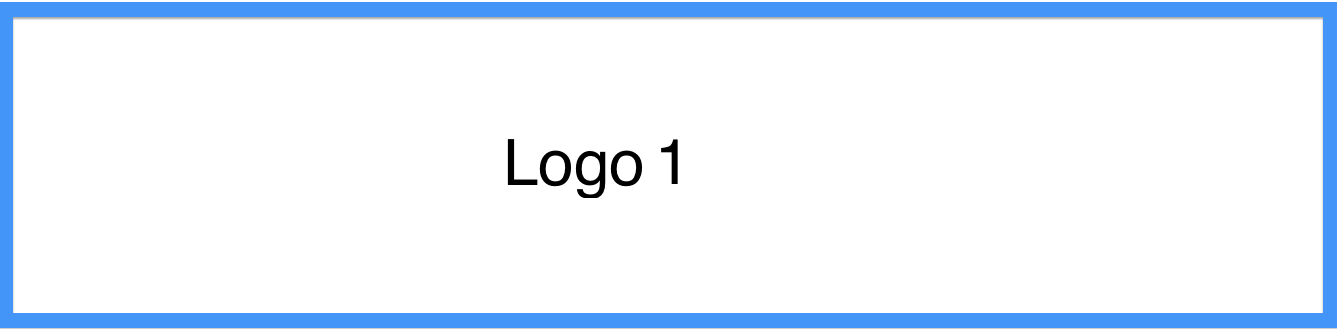
\includegraphics[width=0.4\textwidth,angle=45]{abb/logo1}
% \caption[Beispiel einer Bildbeschreibung]{Beispiel einer Bildbeschreibung\footnotemark}
%\label{fig:beispiel1}
%\end{figure}
%\footnotetext{Bildquelle: Beispielquelle}

% Beispiel für Bildintegration
%\begin{figure}[htb]
% \centering
% 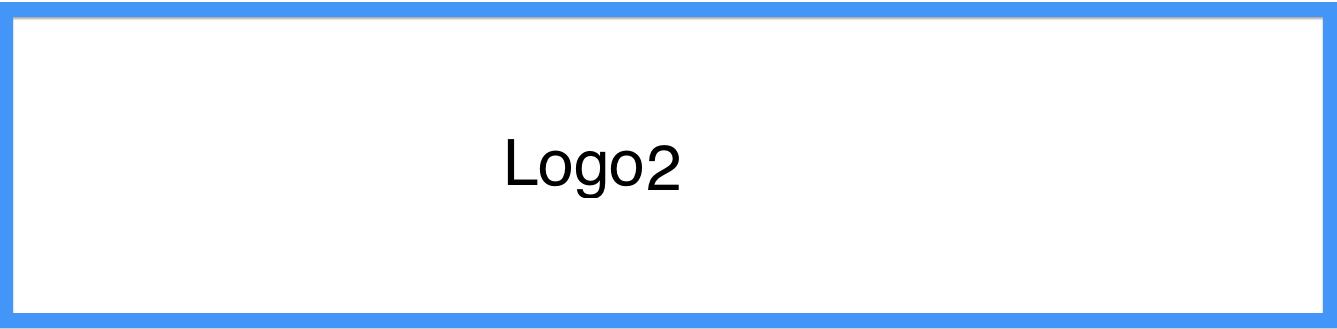
\includegraphics[width=0.3\textwidth,angle=0]{abb/logo2}
% \caption[Beschreibung]{Beschreibung}
%\label{fig:Beschreibung}
%\end{figure}

% Beispiel: Referenz auf Abbildung
Abbildung~\ref{fig:Beschreibung} [S.\pageref{fig:Beschreibung}]

% Beispiel: Tabelle 
\begin{center}
  \begin{tabular}{ | l | c | }
    \hline
    Überschrift 1 & Überschrift 2 \\ \hline \hline
    Info 1 & Info 2 \\ \hline
    Info 3 & Info 4 \\
    \hline
  \end{tabular}
\end{center}


% Beispiel für Quellcode Listings
\lstset{language=xml}
\begin{lstlisting}[frame=htrbl, caption={Die Datei {\tt data-config.xml} dient als Beispiel für XML Quellcode}, label={lst:dataconfigxml}]
<dataConfig>
  <dataSource type="JdbcDataSource" 
              driver="com.mysql.jdbc.Driver"
              url="jdbc:mysql://localhost/bms_db"
              user="root" 
              password=""/>
  <document>
    <entity name="id"
        query="select id, htmlBody, sentDate, sentFrom, subject, textBody
        from mail">
    <field column="id" name="id"/>
    <field column="htmlBody" name="text"/>
    <field column="sentDate" name="sentDate"/>
    <field column="sentFrom" name="sentFrom"/>
    <field column="subject"  name="subject"/>
    <field column="textBody" name="text"/>
    </entity>
  </document>
</dataConfig>
\end{lstlisting}

\lstset{language=java}
\begin{lstlisting}[frame=htrbl, caption={Das Listing zeigt Java Quellcode}, label={lst:result2}]
/* generate TagCloud */
Cloud cloud = new Cloud();
cloud.setMaxWeight(_maxSizeOfText);
cloud.setMinWeight(_minSizeOfText);
cloud.setTagCase(Case.LOWER);
	    
/* evaluate context and find additional stopwords */
String query = getContextQuery(_context);
List<String> contextStoplist = new ArrayList<String>();
contextStoplist = getStopwordsFromDB(query);
	    
/* append context stoplist */
while(contextStoplist != null && !contextStoplist.isEmpty())
  _stoplist.add(contextStoplist.remove(0));
	    
/* add cloud filters */
if (_stoplist != null) {
  DictionaryFilter df = new DictionaryFilter(_stoplist);
  cloud.addInputFilter(df);
}
/* remove empty tags */
NonNullFilter<Tag> nnf = new NonNullFilter<Tag>();
cloud.addInputFilter(nnf);

/* set minimum tag length */
MinLengthFilter mlf = new MinLengthFilter(_minTagLength);
cloud.addInputFilter(mlf);

/* add taglist to tagcloud */
cloud.addText(_taglist);

/* set number of shown tags */	    
cloud.setMaxTagsToDisplay(_tagsToDisplay);
\end{lstlisting}


% Beispiel für Formeln
Die Zuordnung aller möglichen Werte, welche eine Zufallsvariable annehmen kann nennt man \emph{Verteilungsfunktion} von $X$.

\begin{quotation}
Die Funktion F: $\mathbb{R} \rightarrow$ [0,1] mit $F(t) = P (X \le t)$ heißt Verteilungsfunktion von $X$.\footnote{Konen, vgl.~\cite{wk05}~[S.55]}
\end{quotation}

\begin{quotation}
Für eine stetige Zufallsvariable $X: \Omega \rightarrow \mathbb{R}$ heißt eine integrierbare, nichtnegative reelle Funktion $w: \mathbb{R} \rightarrow \mathbb{R}$ mit $F(x) = P(X \le x) = \int_{-\infty}^{x} w(t)dt$ die \emph{Dichte} oder \emph{Wahrscheinlichkeitsdichte} der Zufallsvariablen $X$.\footnote{Konen, vgl.~\cite{wk05}~[S.56]}
\end{quotation}


\onecolumn
% einfacher Zeilenabstand
\singlespacing
% Literaturliste soll im Inhaltsverzeichnis auftauchen
\newpage
\addcontentsline{toc}{section}{Literaturverzeichnis}
% Literaturverzeichnis anzeigen
\renewcommand\refname{Literaturverzeichnis}
\bibliography{Hauptdatei}

%% Index soll Stichwortverzeichnis heissen
% \newpage
% % Stichwortverzeichnis soll im Inhaltsverzeichnis auftauchen
% \addcontentsline{toc}{section}{Stichwortverzeichnis}
% \renewcommand{\indexname}{Stichwortverzeichnis}
% % Stichwortverzeichnis endgueltig anzeigen
% \printindex

\onehalfspacing
% evtl. Anhang
\newpage
\addcontentsline{toc}{section}{Anhang}
\fancyhead[L]{Anhang} %Kopfzeile links
\subsection*{Anhang}\label{anhang}


% Eidesstattliche Erklärung
\addcontentsline{toc}{section}{Eidesstattliche Erklärung}
\section*{Erklärung}

\begin{verbatim}

\end{verbatim}

\noindent
\begin{LARGE}Erklärung zur Bachelorarbeit\end{LARGE}
\begin{verbatim}


\end{verbatim}
Ich versichere, die von mir vorgelegte Arbeit selbstständig verfasst zu haben. Alle Stellen, die wörtlich oder sinngemäß aus veröffentlichten oder nicht veröffentlichten Arbeiten anderer entnommen sind, habe ich als entnommen kenntlich gemacht. Sämtliche Quellen und Hilfsmittel, die ich für die Arbeit benutzt habe, sind angegeben. Die Arbeit hat mit gleichem Inhalt bzw. in wesentlichen Teilen noch keiner anderen Prüfungsbehörde vorgelegen.



\begin{displaymath}
% use packages: array
\begin{array}{ll}
Unterschrift:~~~~~~~~~~~~~~~~~~~~~~~~~~~~~~~~~~~~~~~~~~
& Ort, Datum:~~~~~~~~~~~~~~~~~~~~~~~~~~~~~~~~~~~~~~~~~~
\end{array}
\end{displaymath}


% leere Abschlussseite
\newpage
\thispagestyle{empty} % erzeugt Seite ohne Kopf- / Fusszeile
\section*{ }

\end{document}